
\noindent\begin{minipage}{\textwidth}
    \begin{table}[H]
        \centering
        \caption{Hiperparâmetros e Resultados do Melhor Modelo - inception\_v9\_AM\_opt\_aug}
        \vspace{0.2cm}
        \resizebox{\textwidth}{!}{%
            \begin{tabular}{ll | lrrr}
                \hline
                \multicolumn{2}{c|}{\textbf{Hiperparâmetros}} & \multicolumn{4}{c}{\textbf{Métricas por Classe}} \\ \hline
                \textbf{Parâmetro} & \textbf{Valor} & \textbf{Classe} & \textbf{Precisão} & \textbf{Recall} & \textbf{F1-Score} \\ \hline
    Agendador (Patience) & 4 & 31.2 & 0,4136 & 0,6460 & 0,5043 \\ 
Agendador de LR & ReduceLROnPlateau & 31.3 & 0,3350 & 0,3267 & 0,3308 \\ 
Architecture & inception\_v3 & 31.4 & 0,3503 & 0,2619 & 0,2997 \\ 
Aug (Brilho / Contraste) & 0,29 / 0,01 & 32.3 & 0,4777 & 0,3827 & 0,4249 \\ 
Aug (Prob. Espelhamento) & 0,07 & 32.4 & 0,3214 & 0,3103 & 0,3158 \\ 
Aug (Rotação) & 1\$\textasciicircum{}\textbackslash{}circ\$ & 33.3 & 0,3851 & 0,3472 & 0,3651 \\ 
Augmentation (Método) & Basic & 41.4 & 0,3103 & 0,2045 & 0,2466 \\ 
Batch Size & 32 & 41.5 & 0,4857 & 0,4359 & 0,4595 \\ 
Decaimento de Peso (WD) & 0,0000 & 42.4 & 0,3014 & 0,3235 & 0,3121 \\ 
Dropout & 0,5044 & 44.4 & 0,5294 & 0,6207 & 0,5714 \\ 
\cline{3-6} 
Função de Perda & CrossEntropyLoss & \textbf{Média (Macro)} & 0,3910 & 0,3859 & 0,3830 \\ 
Hidden Units & 1024 & \textbf{MCC} & \multicolumn{3}{c}{0,2902} \\ 
Label Smoothing & 0,1000 &  & & &  \\ 
Otimizador & AdamW &  & & &  \\ 
Taxa de Aprendizado (LR) & 1,38e-04 &  & & &  \\ 
Unfreeze Layers & 6 &  & & &  \\ 
            \hline
            \end{tabular}%
        }
    \end{table}

    \begin{figure}[H]
        \centering
        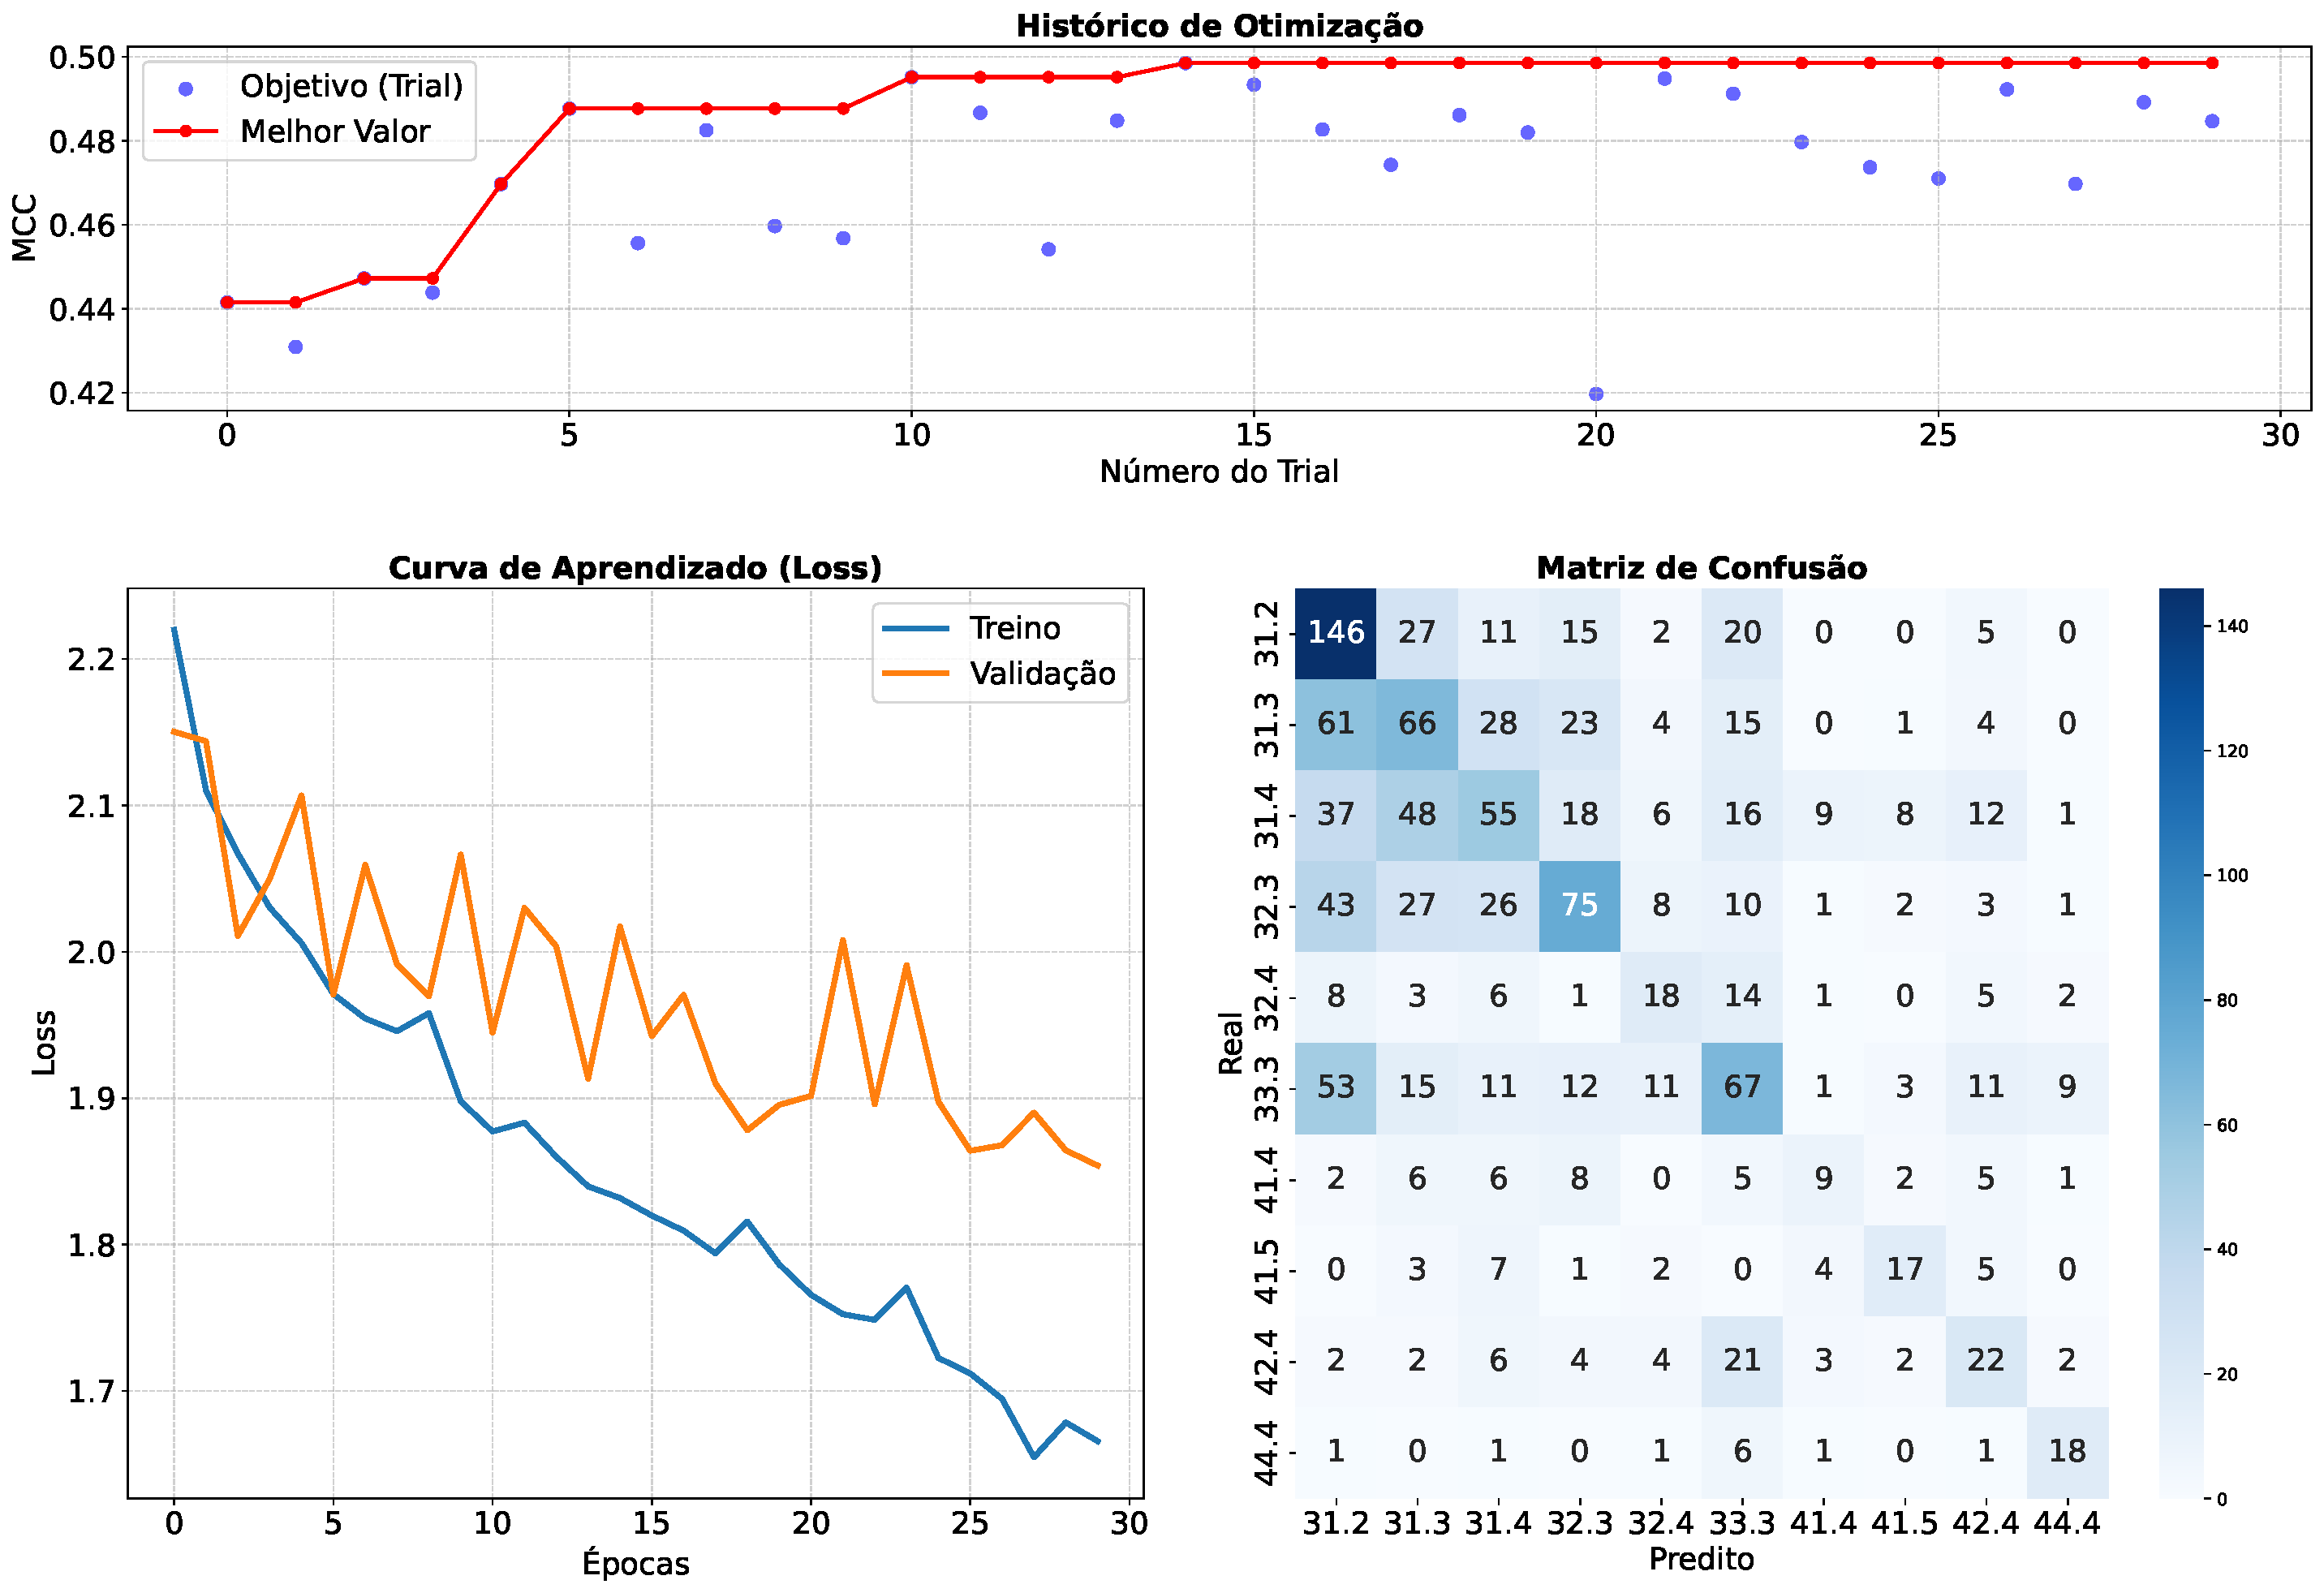
\includegraphics[width=0.85\textwidth]{tex/appendix/experiments/inception_v9_AM_opt_aug/dashboard_consolidado.pdf}
        \caption{Histórico de Otimização, Curvas de Aprendizado e Matriz de Confusão - inception\_v9\_AM\_opt\_aug}
    \end{figure}
\end{minipage}
\clearpage
